\documentclass[]{article}
\usepackage{lmodern}
\usepackage{amssymb,amsmath}
\usepackage{ifxetex,ifluatex}
\usepackage{fixltx2e} % provides \textsubscript
\ifnum 0\ifxetex 1\fi\ifluatex 1\fi=0 % if pdftex
  \usepackage[T1]{fontenc}
  \usepackage[utf8]{inputenc}
\else % if luatex or xelatex
  \ifxetex
    \usepackage{mathspec}
  \else
    \usepackage{fontspec}
  \fi
  \defaultfontfeatures{Ligatures=TeX,Scale=MatchLowercase}
\fi
% use upquote if available, for straight quotes in verbatim environments
\IfFileExists{upquote.sty}{\usepackage{upquote}}{}
% use microtype if available
\IfFileExists{microtype.sty}{%
\usepackage{microtype}
\UseMicrotypeSet[protrusion]{basicmath} % disable protrusion for tt fonts
}{}
\usepackage[margin=1in]{geometry}
\usepackage{hyperref}
\hypersetup{unicode=true,
            pdftitle={Stage 2: Exploratory Data Analysis},
            pdfauthor={Isaac Slagel and Jack Welsh},
            pdfborder={0 0 0},
            breaklinks=true}
\urlstyle{same}  % don't use monospace font for urls
\usepackage{color}
\usepackage{fancyvrb}
\newcommand{\VerbBar}{|}
\newcommand{\VERB}{\Verb[commandchars=\\\{\}]}
\DefineVerbatimEnvironment{Highlighting}{Verbatim}{commandchars=\\\{\}}
% Add ',fontsize=\small' for more characters per line
\usepackage{framed}
\definecolor{shadecolor}{RGB}{248,248,248}
\newenvironment{Shaded}{\begin{snugshade}}{\end{snugshade}}
\newcommand{\KeywordTok}[1]{\textcolor[rgb]{0.13,0.29,0.53}{\textbf{#1}}}
\newcommand{\DataTypeTok}[1]{\textcolor[rgb]{0.13,0.29,0.53}{#1}}
\newcommand{\DecValTok}[1]{\textcolor[rgb]{0.00,0.00,0.81}{#1}}
\newcommand{\BaseNTok}[1]{\textcolor[rgb]{0.00,0.00,0.81}{#1}}
\newcommand{\FloatTok}[1]{\textcolor[rgb]{0.00,0.00,0.81}{#1}}
\newcommand{\ConstantTok}[1]{\textcolor[rgb]{0.00,0.00,0.00}{#1}}
\newcommand{\CharTok}[1]{\textcolor[rgb]{0.31,0.60,0.02}{#1}}
\newcommand{\SpecialCharTok}[1]{\textcolor[rgb]{0.00,0.00,0.00}{#1}}
\newcommand{\StringTok}[1]{\textcolor[rgb]{0.31,0.60,0.02}{#1}}
\newcommand{\VerbatimStringTok}[1]{\textcolor[rgb]{0.31,0.60,0.02}{#1}}
\newcommand{\SpecialStringTok}[1]{\textcolor[rgb]{0.31,0.60,0.02}{#1}}
\newcommand{\ImportTok}[1]{#1}
\newcommand{\CommentTok}[1]{\textcolor[rgb]{0.56,0.35,0.01}{\textit{#1}}}
\newcommand{\DocumentationTok}[1]{\textcolor[rgb]{0.56,0.35,0.01}{\textbf{\textit{#1}}}}
\newcommand{\AnnotationTok}[1]{\textcolor[rgb]{0.56,0.35,0.01}{\textbf{\textit{#1}}}}
\newcommand{\CommentVarTok}[1]{\textcolor[rgb]{0.56,0.35,0.01}{\textbf{\textit{#1}}}}
\newcommand{\OtherTok}[1]{\textcolor[rgb]{0.56,0.35,0.01}{#1}}
\newcommand{\FunctionTok}[1]{\textcolor[rgb]{0.00,0.00,0.00}{#1}}
\newcommand{\VariableTok}[1]{\textcolor[rgb]{0.00,0.00,0.00}{#1}}
\newcommand{\ControlFlowTok}[1]{\textcolor[rgb]{0.13,0.29,0.53}{\textbf{#1}}}
\newcommand{\OperatorTok}[1]{\textcolor[rgb]{0.81,0.36,0.00}{\textbf{#1}}}
\newcommand{\BuiltInTok}[1]{#1}
\newcommand{\ExtensionTok}[1]{#1}
\newcommand{\PreprocessorTok}[1]{\textcolor[rgb]{0.56,0.35,0.01}{\textit{#1}}}
\newcommand{\AttributeTok}[1]{\textcolor[rgb]{0.77,0.63,0.00}{#1}}
\newcommand{\RegionMarkerTok}[1]{#1}
\newcommand{\InformationTok}[1]{\textcolor[rgb]{0.56,0.35,0.01}{\textbf{\textit{#1}}}}
\newcommand{\WarningTok}[1]{\textcolor[rgb]{0.56,0.35,0.01}{\textbf{\textit{#1}}}}
\newcommand{\AlertTok}[1]{\textcolor[rgb]{0.94,0.16,0.16}{#1}}
\newcommand{\ErrorTok}[1]{\textcolor[rgb]{0.64,0.00,0.00}{\textbf{#1}}}
\newcommand{\NormalTok}[1]{#1}
\usepackage{graphicx,grffile}
\makeatletter
\def\maxwidth{\ifdim\Gin@nat@width>\linewidth\linewidth\else\Gin@nat@width\fi}
\def\maxheight{\ifdim\Gin@nat@height>\textheight\textheight\else\Gin@nat@height\fi}
\makeatother
% Scale images if necessary, so that they will not overflow the page
% margins by default, and it is still possible to overwrite the defaults
% using explicit options in \includegraphics[width, height, ...]{}
\setkeys{Gin}{width=\maxwidth,height=\maxheight,keepaspectratio}
\IfFileExists{parskip.sty}{%
\usepackage{parskip}
}{% else
\setlength{\parindent}{0pt}
\setlength{\parskip}{6pt plus 2pt minus 1pt}
}
\setlength{\emergencystretch}{3em}  % prevent overfull lines
\providecommand{\tightlist}{%
  \setlength{\itemsep}{0pt}\setlength{\parskip}{0pt}}
\setcounter{secnumdepth}{0}
% Redefines (sub)paragraphs to behave more like sections
\ifx\paragraph\undefined\else
\let\oldparagraph\paragraph
\renewcommand{\paragraph}[1]{\oldparagraph{#1}\mbox{}}
\fi
\ifx\subparagraph\undefined\else
\let\oldsubparagraph\subparagraph
\renewcommand{\subparagraph}[1]{\oldsubparagraph{#1}\mbox{}}
\fi

%%% Use protect on footnotes to avoid problems with footnotes in titles
\let\rmarkdownfootnote\footnote%
\def\footnote{\protect\rmarkdownfootnote}

%%% Change title format to be more compact
\usepackage{titling}

% Create subtitle command for use in maketitle
\newcommand{\subtitle}[1]{
  \posttitle{
    \begin{center}\large#1\end{center}
    }
}

\setlength{\droptitle}{-2em}

  \title{Stage 2: Exploratory Data Analysis}
    \pretitle{\vspace{\droptitle}\centering\huge}
  \posttitle{\par}
    \author{Isaac Slagel and Jack Welsh}
    \preauthor{\centering\large\emph}
  \postauthor{\par}
      \predate{\centering\large\emph}
  \postdate{\par}
    \date{4/18/2019}

\usepackage{booktabs}
\usepackage{longtable}
\usepackage{array}
\usepackage{multirow}
\usepackage{wrapfig}
\usepackage{float}
\usepackage{colortbl}
\usepackage{pdflscape}
\usepackage{tabu}
\usepackage{threeparttable}
\usepackage{threeparttablex}
\usepackage[normalem]{ulem}
\usepackage{makecell}
\usepackage{xcolor}

\usepackage{float}

\begin{document}
\maketitle

\section{EDA Main Report}\label{eda-main-report}

\subsection{Introduction}\label{introduction}

Our project plans to look into trend in animal treatment in Dallas
animal shelters. Using a dataset containing information on all recent
animals brought into the shelter, we are going to try to answer some of
the following questions. What traits affect a dog's probability of
adoption? Are there seasonal trends in the adoption of different
animals? Are animals who enter the animal shelter with chips more likely
to be returned to their owner? On the table below you can see some of
the variables we are working with in the dataset.

\subsection{Dogs}\label{dogs}

Dogs are the most common animal winding up in the animal shelters which
form our dataset. From our total of 44,194 dogs, 35\% were adopted, 30\%
were returned to owners, 16\% were trasfered, and 15\% were euthanized.
The most common breed of dog in our dataset is the pitbull, with 10,033
being admited to animal shelters in between 10/01/2017 and 04/03/2019.
We are especially interested in how pitbulls are treated within our
datasets as these dogs have an infamous reputation of being overly
agressive. Is it possible that this reputation results in a lower
adoption rate for pitbulls that other breeds?

\paragraph{Pitbulls}\label{pitbulls}

To look into how pitbulls are handled within animal shelters, we decided
to explore how the outcomes of pitbulls may differ from non-pitbulls.
Table 1 describes the differences in outcome rates for non-pitbulls
compared to pitbulls.

\begin{table}[!h]

\caption{\label{tab:pitbull table}Pitbull Outcomes}
\centering
\begin{tabular}{lrr}
\toprule
Outcome & Pitbull (\%) & Non-Pitbull (\%)\\
\midrule
\rowcolor{gray!6}  Adoption & 32.10 & 36.04\\
Euthanized & 28.67 & 10.43\\
\rowcolor{gray!6}  Returned to owner & 22.03 & 31.01\\
Transfer & 10.98 & 17.74\\
\rowcolor{gray!6}  Foster & 2.16 & 1.57\\
\addlinespace
Other & 1.83 & 0.99\\
\rowcolor{gray!6}  Dead on arrival & 0.88 & 0.83\\
Treatment & 0.79 & 0.95\\
\rowcolor{gray!6}  Died & 0.52 & 0.39\\
Missing & 0.04 & 0.06\\
\bottomrule
\end{tabular}
\end{table}

We see that pitbulls, while only adopted at a slightly lower rate
(\textasciitilde{}5\%), are euthanized at well over double the rate of
other dogs. Further, we see that other dogs have a much higher chance of
being trasfered to another facility or returned to their owner. It would
be valuble to get a better understanding of this relationship, but we
likely need to control for things like chip status and intake condition.
Moving foward we would like to look into some binomial regression to
look into the outcomes of pitbulls. To do this we plan to make a more
general outcome variable of Dead or Alive status (to reduce the
dimension of the current outcome\_type variable). In fitting this model
we plan to control for intake status (with which we still need to do
some work on string analysis), chip\_status, and month.

\subsection{Dogs vs Cats}\label{dogs-vs-cats}

In Minnesota and Iowa, our home states, animal shelters often report
having more difficulty dealing with stray cats. There are lots of
problems that feral cats cause including environmental damage and spread
of disease. We were interested if we can see these kinds of differences
in our data. Do cats spend longer in animal shelters? Are they
euthanized at higher rates? To describe some of these differences we
looked we created a summary graph of different characteristics of dogs
and cats. Since our dataset contains observations of 44194 dogs and only
12891 cats, we created this chart in terms of proportion of each animal
matching a certain critera.

\begin{figure}[H]

{\centering 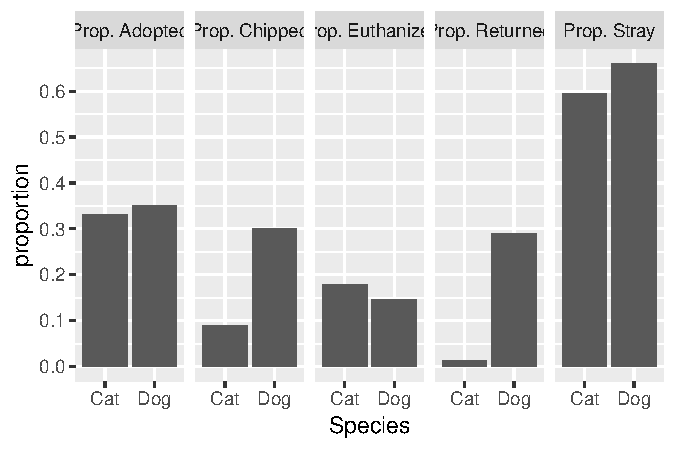
\includegraphics[width=0.6\linewidth]{Stage_2_files/figure-latex/DogCat Figure-1} 

}

\caption{Cat vs Dog Characteristics}\label{fig:DogCat Figure}
\end{figure}

Interestingly enough, we see that the difference between proportions of
cats and dogs adopted is not very pronounced. A slightly lower
percentage of cats are adopted and a slightly higher percent of cats are
euthanized compared to dogs. However, we do see that very few cats
entering humane societys have scannable chips, and an even lower
proportion are returned to their owner. Additionally it seems appears
that fewer cats are brought into the shelter as strays. We may use this
data to do another binomial analysis to piece apart differences between
cat and dog adoptions. We may do a similar thing as the pitbull analysis
with the creation of a dead or alive outcome variable. We would want to
consider controlling for in this analysis would be breed, intake
condition,and chip status.

\subsection{Time of Year}\label{time-of-year}

Another question that we had in our Stage 1 report was what seasonal
trends exists in adoptions. One could imagine a situation where more
puppies are adopted in December or more rabbits are adopted in early
spring. To explore this we did some ploting to see how many animals were
adopted in each months.

\begin{figure}[H]

{\centering 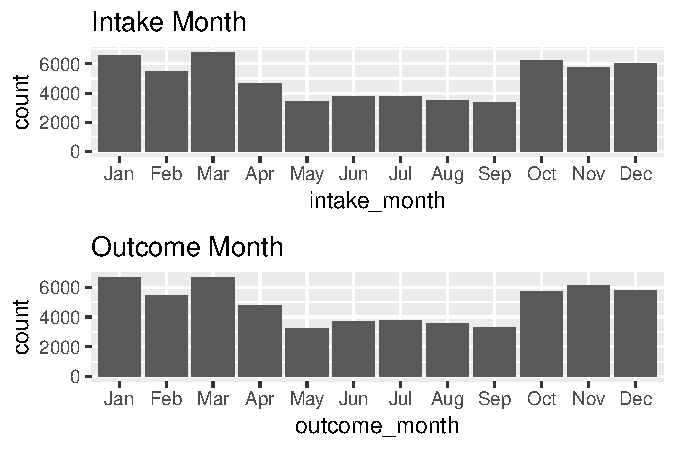
\includegraphics[width=0.6\linewidth]{Stage_2_files/figure-latex/Month Figure-1} 

}

\caption{Animal Adoptions by Month}\label{fig:Month Figure}
\end{figure}

These trends surprised us. We see a large drop in adoptions during the
summer but a spike in the fall, winter, and early spring. These trends
were true for both Dog and Cat adoptions (see appendix). For rabbits,
many were adopted in February and July. While we are unable to put
together a rigourus defense for why these trends are occuring, we see
that we may need to control for it in our binomial analysis.

\pagebreak

\section{Annotated Appendix and
References}\label{annotated-appendix-and-references}

\subsection{Variables}\label{variables}

\begin{table}[!h]

\caption{\label{tab:variable table}Description of Variables}
\centering
\resizebox{\linewidth}{!}{
\begin{tabular}{lll>{\raggedright\arraybackslash}p{4cm}l}
\toprule
Variable Name & Variable Role & Variable Type & Range of Values & Units\\
\midrule
\rowcolor{gray!6}  animal\_breed & explanatory & categorical & 296 unique breeds & NA\\
animal\_origin & explanatory & categorical & 4 sources of shelter animals & NA\\
\rowcolor{gray!6}  animal\_type & explanatory & categorical & 5 species of animal & NA\\
chip\_status & explanatory & bianary & (0,1) & NA\\
\rowcolor{gray!6}  intake\_type & potential confounder & categorial & how animal came to be at the shelter & NA\\
\addlinespace
outcome\_type & reponse & categorial & how animals was removed from shelter & NA\\
\rowcolor{gray!6}  intake\_condition & potential confounder & categorial & keyword description of animal status at intake & NA\\
outcome\_condition & potential confounder & categorial & keyword description of animal status at outcome & NA\\
\rowcolor{gray!6}  intake\_date & response & date & (2017-10-01, 2019-04-03) & y-m-d\\
outcome\_date & response & date & (2017-10-01, 2019-04-03) & y-m-d\\
\bottomrule
\end{tabular}}
\end{table}

\subsection{Citations}\label{citations}

\begin{enumerate}
\def\labelenumi{\arabic{enumi}.}
\item
  \href{https://www.tandfonline.com/doi/abs/10.1207/S15327604JAWS0501_3}{Lepper,
  M., Kass, P. H., \& Hart, L. A. (2002). Prediction of adoption versus
  euthanasia among dogs and cats in a California animal shelter. Journal
  of Applied Animal Welfare Science, 5(1), 29-42.}
\item
  \href{https://europepmc.org/abstract/med/9713528}{Posage, J. M.,
  Bartlett, P. C., \& Thomas, D. K. (1998). Determining factors for
  successful adoption of dogs from an animal shelter. Journal of the
  American Veterinary Medical Association, 213(4), 478-482.}
\item
  \href{https://www.tandfonline.com/doi/abs/10.1080/10888705.2014.982796}{Lampe,
  R., \& Witte, T. H. (2015). Speed of dog adoption: Impact of online
  photo traits. Journal of applied animal welfare science, 18(4),
  343-354.}
\end{enumerate}

\subsection{Exploring animal\_type}\label{exploring-animal_type}

\begin{Shaded}
\begin{Highlighting}[]
\CommentTok{# animal type}
\NormalTok{adoptions }\OperatorTok
\StringTok{  }\KeywordTok{group_by}\NormalTok{(animal_type) }\OperatorTok
\StringTok{  }\KeywordTok{count}\NormalTok{(}\DataTypeTok{sort =} \OtherTok{TRUE}\NormalTok{)}
\end{Highlighting}
\end{Shaded}

\begin{verbatim}
## # A tibble: 6 x 2
## # Groups:   animal_type [6]
##   animal_type     n
##   <chr>       <int>
## 1 DOG         44194
## 2 CAT         12891
## 3 WILDLIFE     1696
## 4 BIRD          485
## 5 LIVESTOCK      33
## 6 D               1
\end{verbatim}

\begin{Shaded}
\begin{Highlighting}[]
\NormalTok{adoptions }\OperatorTok
\StringTok{  }\KeywordTok{filter}\NormalTok{(}\OperatorTok{!}\NormalTok{animal_type}\OperatorTok\KeywordTok{c}\NormalTok{(}\StringTok{"D"}\NormalTok{, }\StringTok{"LIVESTOCK"}\NormalTok{)) }\OperatorTok
\StringTok{  }\KeywordTok{ggplot}\NormalTok{(}\KeywordTok{aes}\NormalTok{(}\DataTypeTok{x=}\NormalTok{animal_type))}\OperatorTok{+}
\StringTok{  }\KeywordTok{geom_bar}\NormalTok{()}
\end{Highlighting}
\end{Shaded}

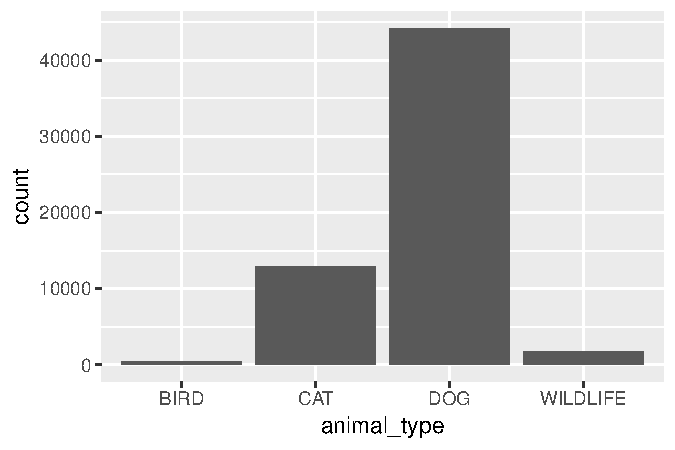
\includegraphics{Stage_2_files/figure-latex/unnamed-chunk-2-1.pdf}

We see that most observations in our dataaset were of dogs, followed by
cats. It seems there is 1 mislabeled dog which we will take care of in
our data cleaning file.

\subsection{Exploring animal\_breed}\label{exploring-animal_breed}

\begin{Shaded}
\begin{Highlighting}[]
\NormalTok{## Which dog breeds are in our data?}
\NormalTok{adoptions }\OperatorTok
\StringTok{  }\KeywordTok{filter}\NormalTok{(animal_type }\OperatorTok{==}\StringTok{ "DOG"}\NormalTok{) }\OperatorTok
\StringTok{  }\KeywordTok{mutate}\NormalTok{(}\DataTypeTok{animal_breed =} \KeywordTok{fct_lump}\NormalTok{(animal_breed, }\DataTypeTok{n=}\DecValTok{15}\NormalTok{)) }\OperatorTok
\StringTok{  }\KeywordTok{group_by}\NormalTok{(animal_breed) }\OperatorTok
\StringTok{  }\KeywordTok{count}\NormalTok{(}\DataTypeTok{sort =} \OtherTok{TRUE}\NormalTok{)}
\end{Highlighting}
\end{Shaded}

\begin{verbatim}
## # A tibble: 16 x 2
## # Groups:   animal_breed [16]
##    animal_breed        n
##    <fct>           <int>
##  1 PIT BULL        10033
##  2 Other            9423
##  3 CHIHUAHUA SH     6322
##  4 GERM SHEPHERD    5625
##  5 LABRADOR RETR    5353
##  6 CAIRN TERRIER    1430
##  7 ALASKAN HUSKY     812
##  8 ROTTWEILER        751
##  9 SHIH TZU          696
## 10 AUST CATTLE DOG   683
## 11 BOXER             629
## 12 DACHSHUND         581
## 13 CHIHUAHUA LH      528
## 14 POODLE MIN        476
## 15 AM PIT BULL TER   433
## 16 BORDER COLLIE     419
\end{verbatim}

\begin{Shaded}
\begin{Highlighting}[]
\NormalTok{adoptions }\OperatorTok
\StringTok{  }\KeywordTok{filter}\NormalTok{(animal_type }\OperatorTok{==}\StringTok{ "DOG"}\NormalTok{) }\OperatorTok
\StringTok{  }\KeywordTok{mutate}\NormalTok{(}\DataTypeTok{animal_breed =} \KeywordTok{fct_lump}\NormalTok{(animal_breed, }\DataTypeTok{n=}\DecValTok{15}\NormalTok{)) }\OperatorTok
\StringTok{  }\KeywordTok{group_by}\NormalTok{(animal_breed) }\OperatorTok
\StringTok{  }\KeywordTok{count}\NormalTok{(}\DataTypeTok{sort =} \OtherTok{TRUE}\NormalTok{)}\OperatorTok
\StringTok{  }\KeywordTok{ggplot}\NormalTok{(}\KeywordTok{aes}\NormalTok{(}\DataTypeTok{x=}\KeywordTok{fct_reorder}\NormalTok{(animal_breed,n), }\DataTypeTok{y=}\NormalTok{n))}\OperatorTok{+}
\StringTok{  }\KeywordTok{geom_bar}\NormalTok{(}\DataTypeTok{stat=}\StringTok{"identity"}\NormalTok{)}\OperatorTok{+}
\StringTok{  }\KeywordTok{coord_flip}\NormalTok{()}
\end{Highlighting}
\end{Shaded}

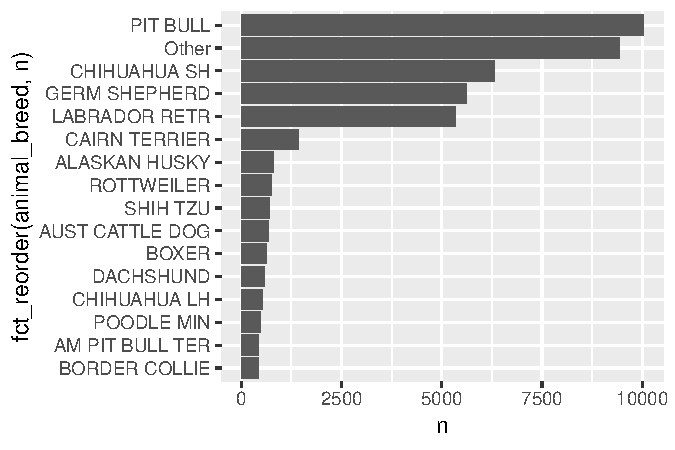
\includegraphics{Stage_2_files/figure-latex/unnamed-chunk-3-1.pdf}

We have a huge variety of dog breeds in our data. The pmost common breed
is the pitbull, which we are planning to use for our analysis. There are
many other dog breeds that are seen as agressive (rottweilers and
boxers) that we may make into a new variable \texttt{aggressive}.

\begin{Shaded}
\begin{Highlighting}[]
\NormalTok{## Which cat breeds are in our data?}
\NormalTok{adoptions }\OperatorTok
\StringTok{  }\KeywordTok{filter}\NormalTok{(animal_type }\OperatorTok{==}\StringTok{ "CAT"}\NormalTok{) }\OperatorTok
\StringTok{  }\KeywordTok{mutate}\NormalTok{(}\DataTypeTok{animal_breed =} \KeywordTok{fct_lump}\NormalTok{(animal_breed, }\DataTypeTok{n=}\DecValTok{10}\NormalTok{)) }\OperatorTok
\StringTok{  }\KeywordTok{group_by}\NormalTok{(animal_breed) }\OperatorTok
\StringTok{  }\KeywordTok{count}\NormalTok{(}\DataTypeTok{sort =} \OtherTok{TRUE}\NormalTok{)}
\end{Highlighting}
\end{Shaded}

\begin{verbatim}
## # A tibble: 11 x 2
## # Groups:   animal_breed [11]
##    animal_breed     n
##    <fct>        <int>
##  1 DOMESTIC SH  11273
##  2 DOMESTIC MH    916
##  3 DOMESTIC LH    219
##  4 SIAMESE        214
##  5 AMER SH        101
##  6 RUSSIAN BLUE    96
##  7 Other           33
##  8 MAINE COON      19
##  9 PERSIAN          8
## 10 AMER CURL SH     6
## 11 BOMBAY           6
\end{verbatim}

\begin{Shaded}
\begin{Highlighting}[]
\NormalTok{adoptions }\OperatorTok
\StringTok{  }\KeywordTok{filter}\NormalTok{(animal_type }\OperatorTok{==}\StringTok{ "CAT"}\NormalTok{) }\OperatorTok
\StringTok{  }\KeywordTok{mutate}\NormalTok{(}\DataTypeTok{animal_breed =} \KeywordTok{fct_lump}\NormalTok{(animal_breed, }\DataTypeTok{n=}\DecValTok{15}\NormalTok{)) }\OperatorTok
\StringTok{  }\KeywordTok{group_by}\NormalTok{(animal_breed) }\OperatorTok
\StringTok{  }\KeywordTok{count}\NormalTok{(}\DataTypeTok{sort =} \OtherTok{TRUE}\NormalTok{)}\OperatorTok
\StringTok{  }\KeywordTok{ggplot}\NormalTok{(}\KeywordTok{aes}\NormalTok{(}\DataTypeTok{x=}\KeywordTok{fct_reorder}\NormalTok{(animal_breed,n), }\DataTypeTok{y=}\NormalTok{n))}\OperatorTok{+}
\StringTok{  }\KeywordTok{geom_bar}\NormalTok{(}\DataTypeTok{stat=}\StringTok{"identity"}\NormalTok{)}\OperatorTok{+}
\StringTok{  }\KeywordTok{coord_flip}\NormalTok{()}
\end{Highlighting}
\end{Shaded}

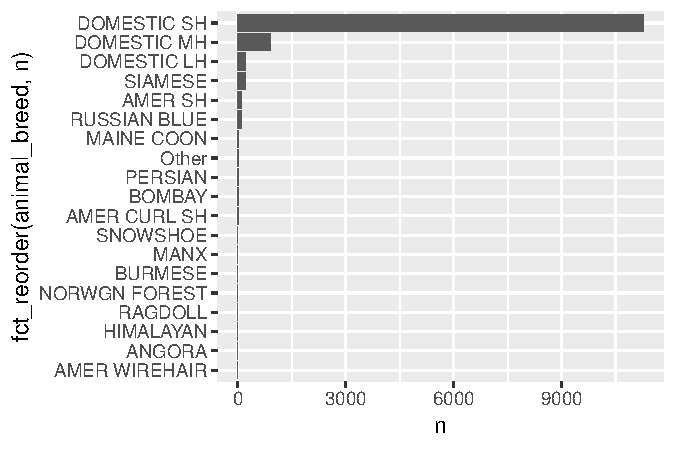
\includegraphics{Stage_2_files/figure-latex/unnamed-chunk-4-1.pdf}

Almost all of the cats in our data were domestic short hair cats.

\begin{Shaded}
\begin{Highlighting}[]
\NormalTok{## Which types of wildlife are in our data?}
\NormalTok{adoptions }\OperatorTok
\StringTok{  }\KeywordTok{filter}\NormalTok{(animal_type }\OperatorTok{==}\StringTok{ "WILDLIFE"}\NormalTok{) }\OperatorTok
\StringTok{  }\KeywordTok{mutate}\NormalTok{(}\DataTypeTok{animal_breed =} \KeywordTok{fct_lump}\NormalTok{(animal_breed, }\DataTypeTok{n=}\DecValTok{10}\NormalTok{)) }\OperatorTok
\StringTok{  }\KeywordTok{group_by}\NormalTok{(animal_breed) }\OperatorTok
\StringTok{  }\KeywordTok{count}\NormalTok{(}\DataTypeTok{sort =} \OtherTok{TRUE}\NormalTok{)}
\end{Highlighting}
\end{Shaded}

\begin{verbatim}
## # A tibble: 11 x 2
## # Groups:   animal_breed [11]
##    animal_breed     n
##    <fct>        <int>
##  1 RACCOON        471
##  2 OPOSSUM        404
##  3 TURTLE         190
##  4 GUINEA PIG     148
##  5 RABBIT SH      136
##  6 HAMSTER         98
##  7 SQUIRREL        82
##  8 Other           68
##  9 BAT             59
## 10 FOX             23
## 11 SKUNK           17
\end{verbatim}

This variable is more for fun. Look at all these fun creatures they get
to deal with at the animal shelter. We are kind of interested in rabbits
so we will talk about that later.

\subsection{Exploring animal origin}\label{exploring-animal-origin}

\begin{Shaded}
\begin{Highlighting}[]
\NormalTok{adoptions }\OperatorTok
\StringTok{  }\KeywordTok{filter}\NormalTok{(dog }\OperatorTok{==}\StringTok{ }\DecValTok{1} \OperatorTok{|}\StringTok{ }\NormalTok{cat }\OperatorTok{==}\StringTok{ }\DecValTok{1}\NormalTok{) }\OperatorTok
\StringTok{  }\KeywordTok{filter}\NormalTok{(}\OperatorTok{!}\KeywordTok{is.na}\NormalTok{(animal_origin)) }\OperatorTok
\StringTok{  }\KeywordTok{ggplot}\NormalTok{(}\KeywordTok{aes}\NormalTok{(}\DataTypeTok{x=}\NormalTok{animal_origin))}\OperatorTok{+}
\StringTok{  }\KeywordTok{geom_bar}\NormalTok{()}\OperatorTok{+}
\StringTok{  }\KeywordTok{facet_grid}\NormalTok{(}\OperatorTok{~}\NormalTok{animal_type)}
\end{Highlighting}
\end{Shaded}

\includegraphics{Stage_2_files/figure-latex/unnamed-chunk-6-1.pdf}

Dogs and cats can come from a 3 possible origins: field, over the
counter, and sweep. As of this moment, we are not sure what the
difference between field and sweep are. However, it is interesting that
only dogs are brought in from sweeps.

\subsection{Exploring chip status}\label{exploring-chip-status}

\begin{Shaded}
\begin{Highlighting}[]
\NormalTok{## General distribution of variable}
\NormalTok{adoptions }\OperatorTok
\StringTok{  }\KeywordTok{filter}\NormalTok{(dog }\OperatorTok{==}\StringTok{ }\DecValTok{1} \OperatorTok{|}\StringTok{ }\NormalTok{cat }\OperatorTok{==}\StringTok{ }\DecValTok{1}\NormalTok{) }\OperatorTok
\StringTok{  }\KeywordTok{ggplot}\NormalTok{(}\KeywordTok{aes}\NormalTok{(}\DataTypeTok{x=}\NormalTok{chip_status))}\OperatorTok{+}
\StringTok{  }\KeywordTok{geom_bar}\NormalTok{()}\OperatorTok{+}
\StringTok{  }\KeywordTok{facet_grid}\NormalTok{(}\OperatorTok{~}\NormalTok{animal_type)}
\end{Highlighting}
\end{Shaded}

\includegraphics{Stage_2_files/figure-latex/unnamed-chunk-7-1.pdf}

\begin{Shaded}
\begin{Highlighting}[]
\NormalTok{## Relationship with returned to owner status}
\NormalTok{adoptions }\OperatorTok
\StringTok{  }\KeywordTok{filter}\NormalTok{(dog }\OperatorTok{==}\StringTok{ }\DecValTok{1} \OperatorTok{|}\StringTok{ }\NormalTok{cat }\OperatorTok{==}\StringTok{ }\DecValTok{1}\NormalTok{) }\OperatorTok
\StringTok{  }\KeywordTok{filter}\NormalTok{(}\OperatorTok{!}\KeywordTok{is.na}\NormalTok{(chip_status)) }\OperatorTok
\StringTok{  }\KeywordTok{mutate}\NormalTok{(}\DataTypeTok{returned =} \KeywordTok{as.factor}\NormalTok{(}\KeywordTok{ifelse}\NormalTok{(outcome_type}\OperatorTok{==}\StringTok{ "RETURNED TO OWNER"}\NormalTok{, }\DecValTok{1}\NormalTok{, }\DecValTok{0}\NormalTok{))) }\OperatorTok
\StringTok{  }\KeywordTok{ggplot}\NormalTok{(}\KeywordTok{aes}\NormalTok{(}\DataTypeTok{x=}\NormalTok{chip_status, }\DataTypeTok{fill =}\NormalTok{ returned))}\OperatorTok{+}
\StringTok{  }\KeywordTok{geom_bar}\NormalTok{(}\DataTypeTok{position =} \StringTok{"fill"}\NormalTok{)}\OperatorTok{+}
\StringTok{  }\KeywordTok{facet_grid}\NormalTok{(}\OperatorTok{~}\NormalTok{animal_type)}
\end{Highlighting}
\end{Shaded}

\includegraphics{Stage_2_files/figure-latex/unnamed-chunk-7-2.pdf}

We see that most cats and dogs do not have chips. However, a larger
proportion of dogs have chips than cats.

A higher proportion of dogs are returned to owners than cats in all
three categories of chip status.

\subsection{Exploring intake\_subtype}\label{exploring-intake_subtype}

\begin{Shaded}
\begin{Highlighting}[]
\NormalTok{## Which dog breeds are in our data?}
\NormalTok{adoptions }\OperatorTok
\StringTok{  }\KeywordTok{mutate}\NormalTok{(}\DataTypeTok{intake_subtype =} \KeywordTok{fct_lump}\NormalTok{(intake_subtype, }\DataTypeTok{n=}\DecValTok{10}\NormalTok{)) }\OperatorTok
\StringTok{  }\KeywordTok{group_by}\NormalTok{(intake_subtype) }\OperatorTok
\StringTok{  }\KeywordTok{count}\NormalTok{(}\DataTypeTok{sort =} \OtherTok{TRUE}\NormalTok{)}
\end{Highlighting}
\end{Shaded}

\begin{verbatim}
## # A tibble: 11 x 2
## # Groups:   intake_subtype [11]
##    intake_subtype           n
##    <fct>                <int>
##  1 AT LARGE             28889
##  2 GENERAL              15495
##  3 CONFINED              5598
##  4 POSSIBLY OWNED        2085
##  5 Other                 1813
##  6 QUARANTINE            1454
##  7 RETURN30              1312
##  8 INJURED                972
##  9 KEEP SAFE              781
## 10 UNINJURED              474
## 11 EUTHANASIA REQUESTED   427
\end{verbatim}

This general intake listing does not give us a lot of infomration.
However we do see that a few animals may have been returned
(non-independent observation), and some animals are requested to be
euthanized upon admission.

\subsection{Exploring intake\_date and
outcome\_date}\label{exploring-intake_date-and-outcome_date}

\begin{Shaded}
\begin{Highlighting}[]
\NormalTok{intake <-}\StringTok{ }\NormalTok{adoptions }\OperatorTok
\StringTok{  }\KeywordTok{mutate}\NormalTok{(}\DataTypeTok{intake_month =} \KeywordTok{month}\NormalTok{(intake_date, }\DataTypeTok{label =} \OtherTok{TRUE}\NormalTok{)) }\OperatorTok
\StringTok{  }\KeywordTok{ggplot}\NormalTok{(}\KeywordTok{aes}\NormalTok{(}\DataTypeTok{x=}\NormalTok{intake_month))}\OperatorTok{+}
\StringTok{  }\KeywordTok{geom_bar}\NormalTok{()}\OperatorTok{+}
\StringTok{  }\KeywordTok{ggtitle}\NormalTok{(}\StringTok{"Intake Month"}\NormalTok{)}

\NormalTok{outcome <-}\StringTok{ }\NormalTok{adoptions }\OperatorTok
\StringTok{  }\KeywordTok{filter}\NormalTok{(}\OperatorTok{!}\KeywordTok{is.na}\NormalTok{(outcome_date)) }\OperatorTok
\StringTok{  }\KeywordTok{mutate}\NormalTok{(}\DataTypeTok{outcome_month =} \KeywordTok{month}\NormalTok{(outcome_date, }\DataTypeTok{label =} \OtherTok{TRUE}\NormalTok{)) }\OperatorTok
\StringTok{  }\KeywordTok{ggplot}\NormalTok{(}\KeywordTok{aes}\NormalTok{(}\DataTypeTok{x=}\NormalTok{outcome_month))}\OperatorTok{+}
\StringTok{  }\KeywordTok{geom_bar}\NormalTok{()}\OperatorTok{+}\StringTok{ }\KeywordTok{ggtitle}\NormalTok{(}\StringTok{"Outcome Month"}\NormalTok{)}
\NormalTok{gridExtra}\OperatorTok{::}\KeywordTok{grid.arrange}\NormalTok{(intake, outcome)}
\end{Highlighting}
\end{Shaded}

\includegraphics{Stage_2_files/figure-latex/unnamed-chunk-9-1.pdf}

\begin{Shaded}
\begin{Highlighting}[]
\CommentTok{# Ammount of time spent at the humane society looks to be about the same from month to month.}

\NormalTok{adoptions }\OperatorTok
\StringTok{  }\KeywordTok{mutate}\NormalTok{(}\DataTypeTok{diff_time=}\KeywordTok{difftime}\NormalTok{(outcome_date, intake_date))}\OperatorTok
\StringTok{  }\KeywordTok{select}\NormalTok{(diff_time, month)}\OperatorTok
\StringTok{  }\KeywordTok{ggplot}\NormalTok{(}\KeywordTok{aes}\NormalTok{(}\DataTypeTok{x=}\NormalTok{diff_time))}\OperatorTok{+}
\StringTok{  }\KeywordTok{geom_density}\NormalTok{()}\OperatorTok{+}
\StringTok{  }\KeywordTok{facet_wrap}\NormalTok{(}\OperatorTok{~}\KeywordTok{as.factor}\NormalTok{(month))}
\end{Highlighting}
\end{Shaded}

\begin{verbatim}
## Don't know how to automatically pick scale for object of type difftime. Defaulting to continuous.
\end{verbatim}

\begin{verbatim}
## Warning: Removed 642 rows containing non-finite values (stat_density).
\end{verbatim}

\includegraphics{Stage_2_files/figure-latex/unnamed-chunk-10-1.pdf}

\subsubsection{Differences in income
day}\label{differences-in-income-day}

\begin{Shaded}
\begin{Highlighting}[]
\NormalTok{adoptions}\OperatorTok
\StringTok{  }\KeywordTok{mutate}\NormalTok{(}\DataTypeTok{out_day=}\KeywordTok{day}\NormalTok{(outcome_date))}\OperatorTok
\StringTok{  }\KeywordTok{ggplot}\NormalTok{(}\KeywordTok{aes}\NormalTok{(}\DataTypeTok{x=}\NormalTok{out_day))}\OperatorTok{+}
\StringTok{  }\KeywordTok{geom_bar}\NormalTok{()}\OperatorTok{+}\StringTok{ }\KeywordTok{ggtitle}\NormalTok{(}\StringTok{"Outcome day"}\NormalTok{)}
\end{Highlighting}
\end{Shaded}

\begin{verbatim}
## Warning: Removed 642 rows containing non-finite values (stat_count).
\end{verbatim}

\includegraphics{Stage_2_files/figure-latex/unnamed-chunk-11-1.pdf}

\begin{Shaded}
\begin{Highlighting}[]
\NormalTok{adoptions}\OperatorTok
\StringTok{  }\KeywordTok{mutate}\NormalTok{(}\DataTypeTok{in_day=}\KeywordTok{day}\NormalTok{(intake_date))}\OperatorTok
\StringTok{  }\KeywordTok{ggplot}\NormalTok{(}\KeywordTok{aes}\NormalTok{(}\DataTypeTok{x=}\NormalTok{in_day))}\OperatorTok{+}
\StringTok{  }\KeywordTok{geom_bar}\NormalTok{()}\OperatorTok{+}\StringTok{ }\KeywordTok{ggtitle}\NormalTok{(}\StringTok{"Outcome day"}\NormalTok{)}
\end{Highlighting}
\end{Shaded}

\includegraphics{Stage_2_files/figure-latex/unnamed-chunk-11-2.pdf}

\subsection{Pitbulls and Adoptions}\label{pitbulls-and-adoptions}

\begin{Shaded}
\begin{Highlighting}[]
\NormalTok{adoptions }\OperatorTok
\StringTok{  }\KeywordTok{filter}\NormalTok{(dog }\OperatorTok{==}\StringTok{ }\DecValTok{1}\NormalTok{) }\OperatorTok
\StringTok{  }\KeywordTok{mutate}\NormalTok{(}\DataTypeTok{adopted =} \KeywordTok{as.factor}\NormalTok{(adopted),}
         \DataTypeTok{pitbull =} \KeywordTok{as.factor}\NormalTok{(pitbull)) }\OperatorTok
\StringTok{  }\KeywordTok{ggplot}\NormalTok{(}\KeywordTok{aes}\NormalTok{(}\DataTypeTok{x =}\NormalTok{ pitbull, }\DataTypeTok{fill =}\NormalTok{ adopted))}\OperatorTok{+}
\StringTok{  }\KeywordTok{geom_bar}\NormalTok{(}\DataTypeTok{position =} \StringTok{"fill"}\NormalTok{)}
\end{Highlighting}
\end{Shaded}

\includegraphics{Stage_2_files/figure-latex/unnamed-chunk-12-1.pdf}

There does not seem to be a large difference between the adoption rates
of pitbull and non-pitbulls. We should try and filter out some of the
non-adopted dogs though, not all dogs come to the shelter to be adopted.

\begin{Shaded}
\begin{Highlighting}[]
\NormalTok{adoptions }\OperatorTok
\StringTok{  }\KeywordTok{filter}\NormalTok{(dog }\OperatorTok{==}\StringTok{ }\DecValTok{1}\NormalTok{) }\OperatorTok
\StringTok{  }\KeywordTok{mutate}\NormalTok{(}\DataTypeTok{euthanized =} \KeywordTok{as.factor}\NormalTok{(euthanized),}
         \DataTypeTok{pitbull =} \KeywordTok{as.factor}\NormalTok{(pitbull)) }\OperatorTok
\StringTok{  }\KeywordTok{ggplot}\NormalTok{(}\KeywordTok{aes}\NormalTok{(}\DataTypeTok{x =}\NormalTok{ pitbull, }\DataTypeTok{fill =}\NormalTok{ euthanized))}\OperatorTok{+}
\StringTok{  }\KeywordTok{geom_bar}\NormalTok{(}\DataTypeTok{position =} \StringTok{"fill"}\NormalTok{)}
\end{Highlighting}
\end{Shaded}

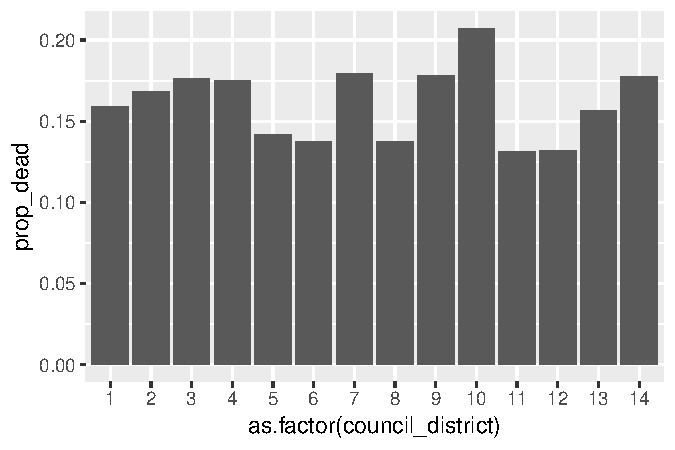
\includegraphics{Stage_2_files/figure-latex/unnamed-chunk-13-1.pdf}

While pitbulls are not adopted at a higher rate, the are euthanized at a
higher rate than other dogs. Lets look at all possible outcomes to see
how this is possible.

\begin{Shaded}
\begin{Highlighting}[]
\NormalTok{adoptions }\OperatorTok
\StringTok{  }\KeywordTok{filter}\NormalTok{(dog }\OperatorTok{==}\StringTok{ }\DecValTok{1}\NormalTok{) }\OperatorTok
\StringTok{  }\KeywordTok{mutate}\NormalTok{(}\DataTypeTok{outcome =} \KeywordTok{as.factor}\NormalTok{(outcome_type),}
         \DataTypeTok{pitbull =} \KeywordTok{as.factor}\NormalTok{(pitbull)) }\OperatorTok
\StringTok{  }\KeywordTok{ggplot}\NormalTok{(}\KeywordTok{aes}\NormalTok{(}\DataTypeTok{x =}\NormalTok{ pitbull, }\DataTypeTok{fill =}\NormalTok{ outcome))}\OperatorTok{+}
\StringTok{  }\KeywordTok{geom_bar}\NormalTok{(}\DataTypeTok{position =} \StringTok{"fill"}\NormalTok{)}
\end{Highlighting}
\end{Shaded}

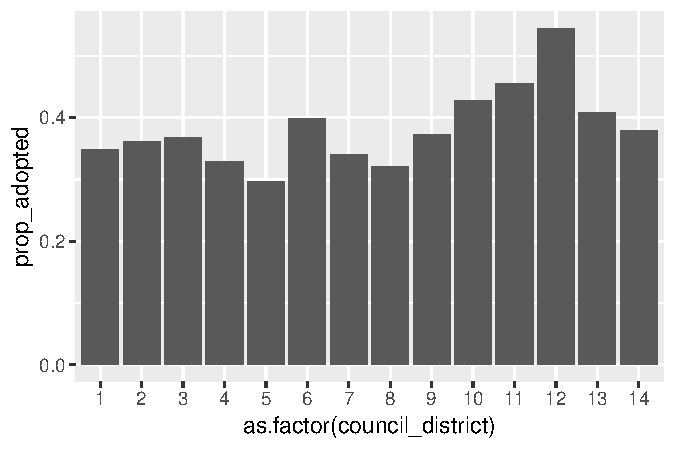
\includegraphics{Stage_2_files/figure-latex/unnamed-chunk-14-1.pdf}

\begin{Shaded}
\begin{Highlighting}[]
\NormalTok{adoptions }\OperatorTok
\StringTok{  }\KeywordTok{filter}\NormalTok{(dog }\OperatorTok{==}\StringTok{ }\DecValTok{1}\NormalTok{) }\OperatorTok
\StringTok{  }\KeywordTok{mutate}\NormalTok{(}\DataTypeTok{outcome =} \KeywordTok{as.factor}\NormalTok{(outcome_type),}
         \DataTypeTok{pitbull =} \KeywordTok{as.factor}\NormalTok{(pitbull)) }\OperatorTok
\StringTok{  }\KeywordTok{group_by}\NormalTok{(pitbull, outcome_type) }\OperatorTok
\StringTok{  }\KeywordTok{count}\NormalTok{() }\OperatorTok
\StringTok{  }\KeywordTok{rename}\NormalTok{(}\StringTok{"freq"}\NormalTok{=n)}\OperatorTok
\StringTok{  }\KeywordTok{group_by}\NormalTok{(pitbull)}\OperatorTok
\StringTok{  }\KeywordTok{mutate}\NormalTok{(}\DataTypeTok{freq =}\NormalTok{ freq}\OperatorTok{/}\StringTok{ }\KeywordTok{sum}\NormalTok{(freq))}\OperatorTok
\StringTok{  }\KeywordTok{spread}\NormalTok{(outcome_type,freq)}
\end{Highlighting}
\end{Shaded}

\begin{verbatim}
## # A tibble: 2 x 11
## # Groups:   pitbull [2]
##   pitbull ADOPTION `DEAD ON ARRIVA~    DIED EUTHANIZED FOSTER MISSING
##   <fct>      <dbl>            <dbl>   <dbl>      <dbl>  <dbl>   <dbl>
## 1 0          0.360          0.00831 0.00386      0.104 0.0157 6.15e-4
## 2 1          0.321          0.00877 0.00518      0.287 0.0216 3.99e-4
## # ... with 4 more variables: OTHER <dbl>, `RETURNED TO OWNER` <dbl>,
## #   TRANSFER <dbl>, TREATMENT <dbl>
\end{verbatim}

A far higher percentage of pitbulls are euthanized than other breeds.
Other dogs are adopted, returned to owners, and trasfered at a higher
rate.

\subsection{Differences between dogs and
cats}\label{differences-between-dogs-and-cats}

\begin{Shaded}
\begin{Highlighting}[]
\NormalTok{adoptions }\OperatorTok
\StringTok{  }\KeywordTok{filter}\NormalTok{(dog }\OperatorTok{==}\StringTok{ }\DecValTok{1} \OperatorTok{|}\StringTok{ }\NormalTok{cat }\OperatorTok{==}\StringTok{ }\DecValTok{1}\NormalTok{) }\OperatorTok
\StringTok{  }\KeywordTok{mutate}\NormalTok{(}\DataTypeTok{Species =} \KeywordTok{ifelse}\NormalTok{(dog }\OperatorTok{==}\StringTok{ }\DecValTok{1}\NormalTok{, }\StringTok{"Dog"}\NormalTok{, }\StringTok{"Cat"}\NormalTok{)) }\OperatorTok
\StringTok{  }\KeywordTok{mutate}\NormalTok{(}\DataTypeTok{returned =} \KeywordTok{ifelse}\NormalTok{(outcome_type }\OperatorTok{==}\StringTok{ "RETURNED TO OWNER"}\NormalTok{, }\DecValTok{1}\NormalTok{, }\DecValTok{0}\NormalTok{)) }\OperatorTok
\StringTok{  }\KeywordTok{group_by}\NormalTok{(Species) }\OperatorTok
\StringTok{  }\KeywordTok{summarise}\NormalTok{(}\DataTypeTok{count =} \KeywordTok{n}\NormalTok{(),}
            \DataTypeTok{meanDays =} \KeywordTok{mean}\NormalTok{(shelter_days, }\DataTypeTok{na.rm =} \OtherTok{TRUE}\NormalTok{),}
            \StringTok{`}\DataTypeTok{Proportion Euthanized}\StringTok{`}\NormalTok{ =}\StringTok{ }\KeywordTok{sum}\NormalTok{(euthanized)}\OperatorTok{/}\NormalTok{count,}
            \StringTok{`}\DataTypeTok{Proportion Adopted}\StringTok{`}\NormalTok{ =}\StringTok{ }\KeywordTok{sum}\NormalTok{(adopted)}\OperatorTok{/}\NormalTok{count,}
            \StringTok{`}\DataTypeTok{Proportion Stray}\StringTok{`}\NormalTok{ =}\StringTok{ }\KeywordTok{sum}\NormalTok{(stray)}\OperatorTok{/}\NormalTok{count,}
           \StringTok{`}\DataTypeTok{Proportion Returned}\StringTok{`}\NormalTok{ =}\StringTok{ }\KeywordTok{sum}\NormalTok{(returned)}\OperatorTok{/}\NormalTok{count,}
           \StringTok{`}\DataTypeTok{Proportion Chipped}\StringTok{`}\NormalTok{ =}\StringTok{ }\KeywordTok{sum}\NormalTok{(chip_status }\OperatorTok{==}\StringTok{ "SCAN CHIP"}\NormalTok{, }\DataTypeTok{na.rm =} \OtherTok{TRUE}\NormalTok{)}\OperatorTok{/}\NormalTok{count)}\OperatorTok
\StringTok{  }\KeywordTok{gather}\NormalTok{(}\DataTypeTok{key =}\NormalTok{ key, }\DataTypeTok{value =}\NormalTok{ proportion, }\DecValTok{4}\OperatorTok{:}\DecValTok{8}\NormalTok{) }\OperatorTok
\StringTok{  }\KeywordTok{ggplot}\NormalTok{(}\KeywordTok{aes}\NormalTok{(}\DataTypeTok{x=}\NormalTok{Species, }\DataTypeTok{y=}\NormalTok{ proportion)) }\OperatorTok{+}
\StringTok{    }\KeywordTok{geom_bar}\NormalTok{(}\DataTypeTok{stat =} \StringTok{"identity"}\NormalTok{)}\OperatorTok{+}
\StringTok{    }\KeywordTok{facet_grid}\NormalTok{(}\DataTypeTok{cols =} \KeywordTok{vars}\NormalTok{(key))}
\end{Highlighting}
\end{Shaded}

\includegraphics{Stage_2_files/figure-latex/unnamed-chunk-15-1.pdf}

Cats are returned at a much lower rate than dogs. Cats have a much lower
proportion with scannable chips than dogs.

\begin{Shaded}
\begin{Highlighting}[]
\NormalTok{adoptions }\OperatorTok
\StringTok{  }\KeywordTok{filter}\NormalTok{(dog }\OperatorTok{==}\StringTok{ }\DecValTok{1} \OperatorTok{|}\StringTok{ }\NormalTok{cat }\OperatorTok{==}\StringTok{ }\DecValTok{1}\NormalTok{) }\OperatorTok
\StringTok{  }\KeywordTok{filter}\NormalTok{(shelter_days }\OperatorTok{<}\StringTok{ }\DecValTok{25}\NormalTok{) }\OperatorTok
\StringTok{  }\KeywordTok{mutate}\NormalTok{(}\DataTypeTok{DogCat =} \KeywordTok{ifelse}\NormalTok{(dog }\OperatorTok{==}\StringTok{ }\DecValTok{1}\NormalTok{, }\StringTok{"Dog"}\NormalTok{, }\StringTok{"Cat"}\NormalTok{)) }\OperatorTok
\StringTok{  }\KeywordTok{ggplot}\NormalTok{(}\KeywordTok{aes}\NormalTok{(}\DataTypeTok{x=}\NormalTok{shelter_days, }\DataTypeTok{y=}\NormalTok{..density..)) }\OperatorTok{+}
\StringTok{  }\KeywordTok{geom_histogram}\NormalTok{()}\OperatorTok{+}
\StringTok{  }\KeywordTok{facet_grid}\NormalTok{(}\OperatorTok{~}\NormalTok{DogCat)}
\end{Highlighting}
\end{Shaded}

\begin{verbatim}
## `stat_bin()` using `bins = 30`. Pick better value with `binwidth`.
\end{verbatim}

\includegraphics{Stage_2_files/figure-latex/unnamed-chunk-16-1.pdf}

Dogs and cats show similar trends in the number of days until adoptions.

\subsection{What about rabbits?}\label{what-about-rabbits}

\begin{Shaded}
\begin{Highlighting}[]
\NormalTok{adoptions  }\OperatorTok
\StringTok{  }\KeywordTok{filter}\NormalTok{(animal_breed}\OperatorTok{==}\StringTok{ "RABBIT SH"}\NormalTok{) }\OperatorTok
\StringTok{  }\KeywordTok{filter}\NormalTok{(adopted }\OperatorTok{==}\StringTok{ }\DecValTok{1}\NormalTok{) }\OperatorTok
\StringTok{  }\KeywordTok{mutate}\NormalTok{(}\DataTypeTok{month =}\NormalTok{ lubridate}\OperatorTok{::}\KeywordTok{month}\NormalTok{(outcome_date, }\DataTypeTok{label =} \OtherTok{TRUE}\NormalTok{)) }\OperatorTok
\StringTok{  }\KeywordTok{ggplot}\NormalTok{(}\KeywordTok{aes}\NormalTok{(}\DataTypeTok{x=}\NormalTok{month)) }\OperatorTok{+}
\StringTok{  }\KeywordTok{geom_bar}\NormalTok{()}
\end{Highlighting}
\end{Shaded}

\includegraphics{Stage_2_files/figure-latex/unnamed-chunk-17-1.pdf}

Alright, so maybe it is not the case that more rabits are adopted over
easter. Are there trends in dog adoptions?

\begin{Shaded}
\begin{Highlighting}[]
\NormalTok{adoptions  }\OperatorTok
\StringTok{  }\KeywordTok{filter}\NormalTok{(dog }\OperatorTok{==}\StringTok{ }\DecValTok{1} \OperatorTok{|}\StringTok{ }\NormalTok{cat }\OperatorTok{==}\StringTok{ }\DecValTok{1}\NormalTok{) }\OperatorTok
\StringTok{  }\KeywordTok{mutate}\NormalTok{(}\DataTypeTok{DogCat =} \KeywordTok{ifelse}\NormalTok{(dog }\OperatorTok{==}\StringTok{ }\DecValTok{1}\NormalTok{, }\StringTok{"Dog"}\NormalTok{, }\StringTok{"Cat"}\NormalTok{)) }\OperatorTok
\StringTok{  }\KeywordTok{filter}\NormalTok{(adopted }\OperatorTok{==}\StringTok{ }\DecValTok{1}\NormalTok{, }\OperatorTok{!}\KeywordTok{is.na}\NormalTok{(month)) }\OperatorTok
\StringTok{  }\KeywordTok{mutate}\NormalTok{(}\DataTypeTok{month =}\NormalTok{ lubridate}\OperatorTok{::}\KeywordTok{month}\NormalTok{(outcome_date, }\DataTypeTok{label =} \OtherTok{TRUE}\NormalTok{)) }\OperatorTok
\StringTok{  }\KeywordTok{ggplot}\NormalTok{(}\KeywordTok{aes}\NormalTok{(}\DataTypeTok{x=}\NormalTok{month, }\DataTypeTok{y =}\NormalTok{ ..prop.., }\DataTypeTok{group =} \DecValTok{1}\NormalTok{)) }\OperatorTok{+}
\StringTok{  }\KeywordTok{geom_bar}\NormalTok{()}\OperatorTok{+}
\StringTok{  }\KeywordTok{facet_grid}\NormalTok{(}\DataTypeTok{rows =} \KeywordTok{vars}\NormalTok{(DogCat), }\DataTypeTok{switch =} \StringTok{"both"}\NormalTok{)}
\end{Highlighting}
\end{Shaded}

\includegraphics{Stage_2_files/figure-latex/unnamed-chunk-18-1.pdf}

These both seem to follow the trend of fewer adoptions in the summer.


\end{document}
